\scanpage{221}
\mspage{171}

\deleted{Dear Justine}
% typed cancellation: xxxxxxxxxxxx

$\overline{\underline{\mathrm{VI}}}$ \deleted{\uline{\unsure{Localiseurs|Localisation}} \unsure{de} \illegible{1} (\unsure{suite})}. \uline{Critère de} $W_\infty$-\uline{asphéricité par les} $\Omega^{\unsure{-|\bullet}}(X,\unsure{-|*})$.

\uline{1} \unsure{les conditions|les localiseurs|la filtration} \unsure{en|sur} $W_n$.

On va définir, pour $n\in\mathbb N$,

\[
 W_n\subset\operatorname{Fl}(\mathrm{Cat})\unsure{,|{;}}
\]

par les conditions suivantes (où $f:X\to Y$ est une flèche dans $\underline{\overline{\mathrm{Cat}}}$)

\[
 f\in W_0\iff\text{a) }\unsure{\pi_0|\Pi_0}(f)\ \text{bijectif}
\]

 \deleted{\unsure{$\Longleftrightarrow$ b)} le foncteur $F\mapsto f^*F$ des}
   
$\Longleftrightarrow$ \deleted{\unsure{b)}}c) le foncteur $F\mapsto f^*F$ des \inserted{\unsure{pré}}faisceaux d'ensembles \uline{constants} sur $Y$ vers les faisceaux d'ens. constants sur $X$ est pleinement fidèle

\margin{\figure{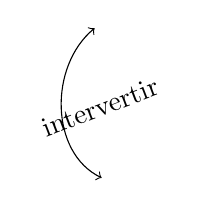
\begin{tikzpicture}
\draw[<->] (0.1,1) .. controls (-0.48,0.52) and (-0.47,-0.58) .. (0.19,-0.9);
\node[rotate=21] at (0.17,0) {\unsure{intervertir}};
\end{tikzpicture}}}
% slanted

$\Longleftrightarrow$ b) Pour tout préfaisceau d'ens. $F$ \uline{constant} sur $Y$,

\[
 H^0(Y,F)\longrightarrow \unsure{H^0|\mathcal H^0}(X,f^*F)\quad\text{est bijectif}
\]

\uline{NB} Si $F_0$ est un ensemble, $F_{0Y}$ le faisceau d'ens. constant défini par $F_0$ sur $Y$, on a

\[
\begin{aligned}
 H^0(Y,F_{0Y})&\simeq\operatorname{Hom}_{\mathrm{ens}}(\pi_0(Y),F_0)
    &&(\text{fonctoriel en }Y)\\
 \operatorname{Hom}_{Y^\wedge}(F_{0Y},G_{0Y})&\simeq
 \operatorname{Hom}_{\mathrm{ens}}(\pi_0(Y),\operatorname{Hom}_{\mathrm{ens}}(F_0,G_0))
    &&(\unsure{\text{id}^{\circ}|\text{id}})
\end{aligned}
\]

ce qui implique que

\[
 a\Longrightarrow \deleted{\unsure{b}}c
\underset{\substack{\text{en prenant}\\\operatorname{Hom}_{Y^\wedge}(e_Y,F)}}{\overset{\text{tautol}}{\Longrightarrow}}
\deleted{\unsure{c}}b\Longrightarrow a.
\]

$f\in W_1\Longleftrightarrow$ a) $\pi_0(f)$ bijectif, et pour tout $x\in\operatorname{Ob}X$,

\[
 \pi_1(f,x):\pi_1(X,x)\mathrel{\unsure{-|\to}}\pi_1(Y,f(x))\quad\text{est bijectif}
\]

(NB Il suffit de le vérifier pour \uline{un} $x$ dans chaque composante connexe de $X$.)

\[
 \text{a') }\Pi(X)\xrightarrow{\Pi f}\Pi(Y)\quad\text{est une équiv. de Cat.}
\]

$\Longleftrightarrow$ b) $H^0(\unsure{Y|X},F)\mathrel{\unsure{-|\to}}H^0(X,f^*(F))$ bijectif pour tout faisceau d'ens. \uline{loc.} \uline{constant} sur $Y$, et $H^1(Y,\deleted{\unsure{G}}F)\to H^1(Y,f^*F)$ bijectif \deleted{pour} \unsure{si} de plus $F$ est un faisceau en groupes.

\inserted{\unsure{b')|bis)} Comme b), mais pour le $H^1$ on se borne à $F$ \uline{constant}, et on exige $H^1(f)$ \uline{surjectif} \unsure{seulemt|seulement}.}

$\Longleftrightarrow$ c) Le foncteur $F\mapsto f^*F$ de la cat. des faisceaux d'ens. loc. constants sur $Y$ vers celle des faisceaux loc. const. sur $X$ est une équiv. de catégories.
% archive sheet number: 221
